\documentclass[11pt,a4paper]{article}

% -------------------------------------------------
% PACKAGES
% -------------------------------------------------
\usepackage[spanish]{babel}
\usepackage[utf8]{inputenc}
\usepackage[T1]{fontenc}
\usepackage{lmodern}
\usepackage[margin=1in]{geometry}

\usepackage{graphicx}
\graphicspath{{./figures/}}
\usepackage{amsmath,amssymb}
\usepackage{booktabs}
\usepackage{xcolor}
\usepackage{hyperref}
\usepackage{fancyhdr}
\usepackage{titlesec}

% -------------------------------------------------
% COLORS
% -------------------------------------------------
\definecolor{primary}{RGB}{25,55,109}

% -------------------------------------------------
% HEADER
% -------------------------------------------------
\pagestyle{fancy}
\fancyhf{}
\fancyhead[L]{Videovigilancia con Interpretación de Escenas}
\fancyfoot[C]{\thepage}

% -------------------------------------------------
% SECTION STYLE
% -------------------------------------------------
\titleformat{\section}
{\large\bfseries\color{primary}}
{\thesection.}{0.5em}{}

% -------------------------------------------------
% DOCUMENT
% -------------------------------------------------
\begin{document}

% =================================================
% TITLE (FULL WIDTH)
% =================================================

\begin{center}

    \vspace{1cm}

    {\Huge\bfseries\color{primary}
        Videovigilancia con Interpretación de Escenas\par}

    \vspace{0.5cm}

    {\Large Analítica de video para seguridad perimetral\par}

    \vspace{0.5cm}

    \large
    \textbf{Autor:} Roberto García Guzmán\\
    \textbf{Institución:} Universidad de Guanajuato\\
    \textbf{Fecha:} \today

    \vspace{0.5cm}

    \rule{0.8\textwidth}{0.5pt}

    \vspace{0.5cm}

\end{center}

\tableofcontents
\newpage

% =================================================
\section{Resumen ejecutivo}


This section introduces the problem context, objectives, and motivation.
You can discuss background information and explain why the topic is relevant.

Lorem ipsum dolor sit amet, consectetur adipiscing elit. Sed do eiusmod tempor
incididunt ut labore et dolore magna aliqua.

% =================================================
\section{Planteamiento del problema}

La seguridad perimetral es un aspecto crítico en la protección de instalaciones, infraestructuras y áreas sensibles. Usualmente incluye elementos como barreras físicas y sistemas electrónicos diseñados para prevenir accesos no autorizados.

Una de las herramientas más efectivas para la protección perimetral es la videovigilancia, que permite monitorear áreas extensas y detectar actividades sospechosas en tiempo real. Sin embargo, si se desea prevenir eventos de seguridad, es necesario contar con un equipo de personas que monitoreen constantemente las cámaras, lo cual puede ser costoso y propenso a errores humanos.

Con el fin de aliviar este inconveniente, se deben implementar sistemas de videovigilancia inteligentes que puedan interpretar las escenas y detectar actividades sospechosas de manera autónoma, alertando a los operadores solo cuando sea necesario.

Bajo este contexto, el objetivo de este proyecto es desarrollar un sistema de videovigilancia autónomo, con la capacidad de interpretar escenas, con el objetivo de mejorar la seguridad perimetral, utilizando técnicas avanzadas de análisis de video e inteligencia artificial.

\subsection{Inteligencia artificial en el análisis de video}

Una de las principales aplicaciones de la inteligencia artificial en el análisis de video en general es la detección de objetos. Esto se refiere a la capacidad de identificar y localizar objetos específicos dentro de un video, como personas, vehículos o animales. Esto se hace a través de algoritmos de aprendizaje profundo, como las redes neuronales convolucionales (CNN), que pueden aprender a reconocer patrones visuales complejos.

En este proyecto, se plantea el uso de una red neuronal convolucional para la detección de objetos relevantes en cada cuadro del video. Una vez detectados estos objetos, se aplicarán técnicas de seguimiento para mantener un registro de su movimiento a lo largo del tiempo. Esto permitirá analizar el comportamiento de los objetos y detectar actividades sospechosas, como intrusión, merodeo o abandono de objetos. Además, se empleará la capacidad de detección de objetos para identificar la presencia de armas de fuego en las escenas.

\subsection{Objetivos}

\begin{itemize}
    \item Desarrollar un algoritmo de análisis de video capaz de detectar cuatro tipos de actividades sospechosas: intrusión, merodeo, abandono de objetos y armas de fuego.
    \item Desarrollar una aplicación web por medio de la cual un usuario pueda configurar el sistema y recibir alertas en tiempo real.
    \item Evaluar el sistema utilizando un conjunto de datos de videovigilancia y medir su precisión, tasa de falsos positivos, tiempo de respuesta y recursos computacionales utilizados.
\end{itemize}

\section{Arquitectura del sistema}

\begin{figure}[h!]
    \centering
    
\includegraphics[width=\linewidth]{general_schema.pdf}
    \caption{Arquitectura general del sistema de videovigilancia con interpretación de escenas.}
    \label{fig:general_schema}
\end{figure}

El sistema propuesto tiene tres componentes principales: el módulo de detección de objetos, el módulo de seguimiento de objetos y el módulo de análisis de la escena. Estos tres componentes procesan la información como se muestra en el diagrama de la figura \ref{fig:general_schema}.

\subsection{Módulo de detección de objetos}

Se entiende por detección al obtener las coordenadas y dimensiones de un objeto en una imagen, usualmente en la forma de cajas de detección con las propiedades: posición en $x$, posición en $y$, ancho y alto. Usualmente, esta detección va acompañada de una clase, que indica el tipo de objeto del que se trata, y un porcentaje de confianza de que la detección es correcta.

Para realizar la detección de los objetos, el módulo de detección emplea el modelo convolucional YOLOX, el cual es capaz de detectar objetos con un bajo costo computacional y en tiempo real. La arquitectura YOLOX, se muestra en la figura \ref{fig:yolox}, y consiste de múltiples capas convolucionales y tres salidas: clase, caja de detección y porcentaje de confianza, referido en este caso como IoU.

\begin{figure}[h!]
    \centering
    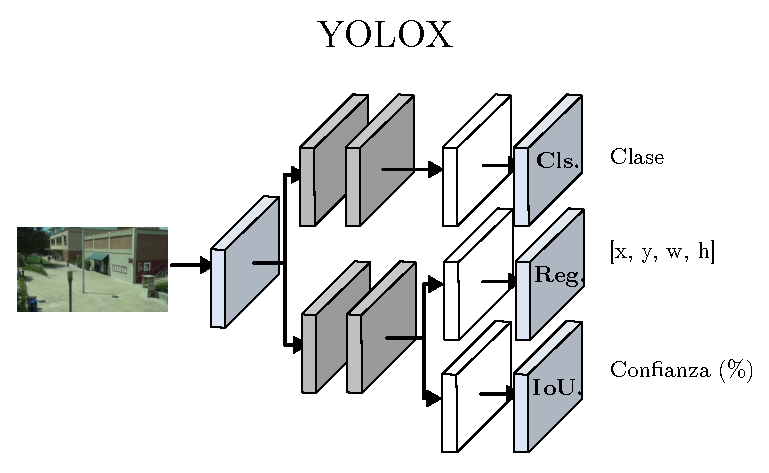
\includegraphics[width=0.5\linewidth]{yolox.pdf}
    \caption{Arquitectura de modelo YOLOX.}
    \label{fig:yolox}
\end{figure}

Para este proyecto se utiliza un modelo YOLOX pre-entrenado en el conjunto de datos COCO 2017. Este conjunto de datos contiene muestras de detección de 80 clases de objetos diferentes. De estas 80 clases, se hace una reducción a 4 clases: personas, vehículos, vehículos ligeros y bolsas. Esta reducción se realiza mediante un mapeo de clases; clases como automovil, autobus o tren, se mapean a la clase vehículos; mientras que clases como bicicleta y motocicleta se mapean a vehículos ligeros. Las demás clases como animales, frutas, etc. son ignoradas aún cuando sean detectadas por el modelo.

El modelo YOLOX tiene variantes tanto para el tamaño de la imagen de entrada, como del número de capas y parámetros. El modelo que se va a emplear en este proyecto es el modelo YOLOX\_s, el cual procesa imágenes de 640x640 pixeles y tiene 9 millones de parámetros.

Además, el proyecto requiere que se pueda detectar objetos como armas de fuego, los cuales no están incluidos en el conjunto de entrenamiento de COCO 2017. Para detectar estos objetos se reentrenó otro modelo YOLOX\_s, en un conjuto de datos de detección de armas.

El módulo de detección de objetos, utiliza ambos modelos sobre cada imagen y combina las detecciones como se muestra en la figura \ref{fig:two_yolox}. Del modelo YOLOX\_s se obtienen 4 clases de objetos, mientras que del modelo YOLOX\_s\_weapon se obtiene una clase adicional de armas de fuego. De esta forma se detectan 5 clases diferentes: personas, vehículos, vehículos ligeros, bolsas y armas de fuego.

\begin{figure}[h!]
    \centering
    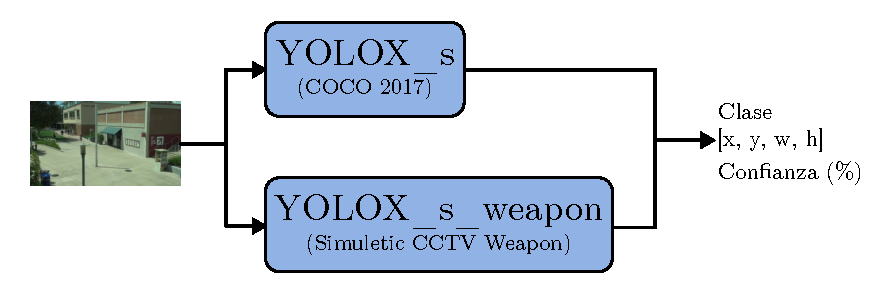
\includegraphics[width=0.7\linewidth]{two_yolox.pdf}
    \caption{Combinación de dos modelos de detección YOLOX\_s.}
    \label{fig:two_yolox}
\end{figure}

\subsection{Módulo de seguimiento de objetos}

El módulo de seguimiento de objetos se encarga de mantener un registro de los objetos detectados a lo largo del tiempo, asignándoles un identificador único. Esto permite analizar el comportamiento de los objetos y detectar actividades sospechosas, como intrusión, merodeo o abandono de objetos. Para realizar el seguimiento de los objetos, se emplea el algoritmo Deep SORT, el cual combina la información de las cajas de detección con características visuales extraídas por una red neuronal para mantener un seguimiento robusto incluso en situaciones de oclusión.

El algoritmo Deep SORT utiliza como entrada las cajas de detección obtenidas del módulo de detección de objetos. Con cada caja, extrae el recorte correspondiente de la imagen original y obtiene un vector de características (o descriptor de apariencia), empleando una red neuronal convolucional. Posteriormente, genera un vector de estado que incluye: posición en $x$, posición en $y$, relación de aspecto $a$, altura $h$, velocidad en $x$, velocidad en $y$, cambio de la relación de aspecto $a$ y cambio de altura $h$. Con esta información aplica un filtro de Kalman para predecir el estado del objeto en la siguiente imagen. Finalmente, utiliza el algoritmo húngaro para emparejar las nuevas detecciones con las de la imagen anterior, utilizando tanto la predicción de estado como el descriptor de apariencia. Este algoritmo se ilustra en la figura \ref{fig:deepsort}.

\begin{figure}[h!]
    \centering
    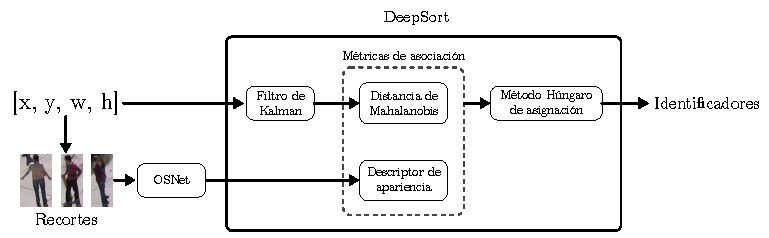
\includegraphics[width=0.9\linewidth]{deepsort.pdf}
    \caption{Algoritmo Deep SORT.}
    \label{fig:deepsort}
\end{figure}

La red neuronal OSNet (Omni-Scale Network) es una red neuronal convolucional profunda diseñada para realizar re-identificación de personas. Esta tarea requiere encontrar características discriminativas que pudan distinguir individuos entre diferentes ángulos de la cámara.

\subsection{Módulo de análisis de la escena}

Este módulo es el encargado de verificar las posiciones de los objetos y emitir las alarmas cuando se presenten eventos de seguridad.

Los cuatro eventos de seguridad son: Intrusión, merodeo, objetos abandonados y armas. A continuación se explica cómo se detecta cada uno de ellos.

\subsubsection{Intrusión}

Se comienza por generar un polígono que delimita el área restringida, de este polígono se obtiene una máscara del área restringida. Cuando se detecta una persona en la escena, se obtiene su caja de detección y se genera una máscara de detección. Una vez obtenidas ambas máscaras se calcula el área de intersección y se divide entre el área de detección para obtener un porcentaje de intrusión. Si el porcentaje de intrusión supera el porcentaje mínimo establecido, se emite la alarma. Este proceso se ejemplifica en la figura \ref{fig:intrusion}.

Parámetros:

\begin{itemize}
    \item Porcentaje mínimo de intrusión: Qué tanto se sobrepone el cuadro de detección del objeto sobre el polígono.
\end{itemize}

\begin{figure}[h!]
    \centering
    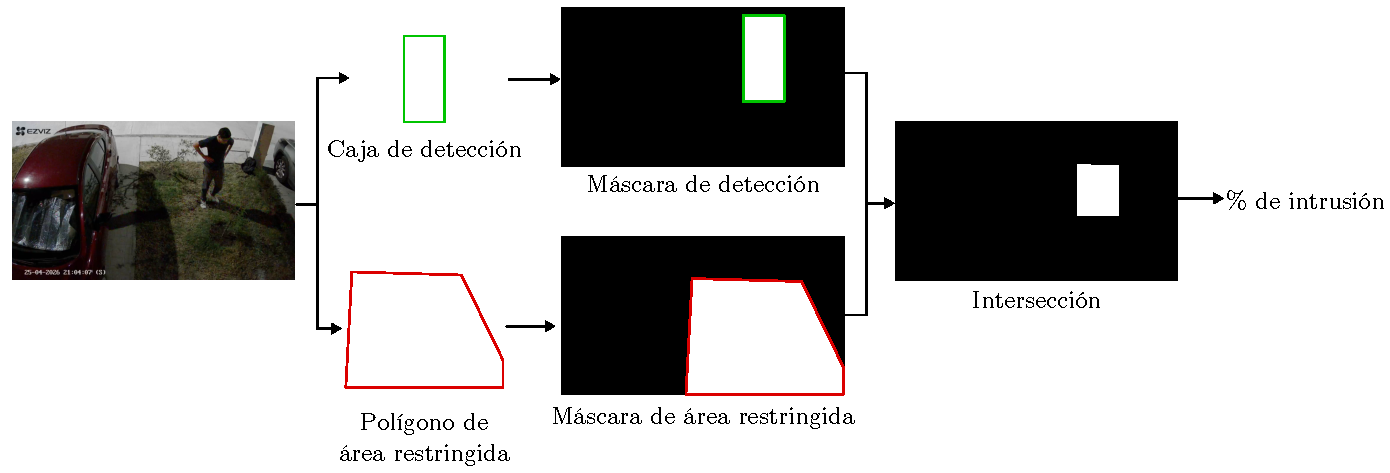
\includegraphics[width=0.9\linewidth]{intrusion.pdf}
    \caption{Algoritmo de detección de intrusiones.}
    \label{fig:intrusion}
\end{figure}

\subsubsection{Merodeo}

Para todos los objetos en la escena que se les asignó un ID, también se almacena un contador que indica el tiempo que ha estado en la escena. Cada vez que se vuelve a detectar el objeto se incrementa este contador con los segundos que pasaron entre un cuadro y otro. Cada cuadro, se verifica este contador y si excede el límite establecido se emite la alarma.

Parámetros:

\begin{itemize}
    \item Tiempo máximo en escena.
\end{itemize}

\subsubsection{Objetos abandonados}

Cada objeto en la escena que se les asignó un ID, además de almacenar el contador de tiempo en escena, se almacena su posición una vez cada segundo, durante los últimos N segundos (por defecto 3600). Al igual que con las personas, se establece un tiempo máximo en escena, una vez superado este límite se calcula la distancia promedio recorrida por el objeto durante los últimos N segundos, si esta distancia es inferior al límite establecido se considera como objeto abandonado y se emite la alarma.

Parámetros.

\begin{itemize}
    \item Tiempo máximo en escena.
    \item Distancia máxima recorrida: Distancia en pixeles en la imagen.
\end{itemize}

Uno de los problemas que nos enfrentamos es que el modelo YOLOX\_s es muy deficiente en la detección de objetos como bolsas o mochilas en imágenes CCTV, ya que están muy lejos de los objetos. Es por ello que se implementó una estrategia alternativa de detección de objetos abandonados.

En esta estrategia primero se debe obtener el fondo de la escena. Para ello, se obtienen los M iniciales frames del video o la captura en tiempo real y se calcula la mediana de cada pixel para obtener una imagen del fondo. Posteriormente, en cada cuadro se calcula la diferencia entre el cuadro y el fondo y se extraen las regiones que difieren, cada region (o contorno) es un posible objeto. Se descartan los objetos que ya fueron detectador por el YOLOX\_s y las regiones faltantes se consideran como objetos con clase \'desconocida\'. Los objetos con clase desconocida se tratan como cualquier otro objeto y se rastrean para la detección de objetos abandonados.

\begin{figure}[h!]
    \centering
    \includegraphics[width=0.9\linewidth]{abandoned_obj.pdf}
    \caption{Algoritmo de obtención de fondo.}
    \label{fig:abandoned_obj_background}
\end{figure}

\begin{figure}[h!]
    \centering
    \includegraphics[width=0.9\linewidth]{abandoned_obj_2.pdf}
    \caption{Algoritmo de detección de objetos desconocidos.}
    \label{fig:abandoned_obj_unknown}
\end{figure}

\subsubsection{Armas de fuego}

La detección de armas de fuego se realiza con el modelo reentrenado YOLOX\_s\_weapon. Para evitar falsos positivos se establce un mínimo de tiempo que el arma debe estar en la escena para que pueda emitirse la alarma.

Parámetros:

\begin{itemize}
    \item Tiempo mínimo
\end{itemize}

\section{Implementación}

El desarrollo del sistema se realizó en Python 3.12 gracias a la variedad de librerías de visión e inteligencia artificial que se encuentran disponibles.

El código se encuentra distribuido en 4 paquetes de python, 3 correspondientes a las librerías de procesamiento de las imágenes y un último paquete que corresponde a la aplicación.

\begin{itemize}
    \item \textbf{yolox:} Paquete para detección de objetos con el modelo YOLOX. Descargado de \url{https://github.com/megvii-basedetection/yolox} y modificado para adaptalo a la versión de Python y al conjunto de datos de armas para entrenamiento.
    \item \textbf{deepsort:} Paquete para el seguimiento de múltiples objetos en video. Descargado de \url{https://github.com/kadirnar/deepsort-pip} y modificado para adaptarlo a la versión de Python y con adiciones para que se integre con el proyecto.
    \item \textbf{yolotracker:} Paquete propio que incluye la lógica de la detección de eventos y combina yolox con deepsort. Este paquete es el principal y contiene todos los algoritmos descritos en la sección anterior.
    \item \textbf{video-surveillance-app:} Contiene la aplicación web para configuración del sistema, así como el servicio que hace la detección de los eventos en tiempo real. No es un paquete de Python en sí.
\end{itemize}

\subsection{Soporte para múltiples cámaras}

Las cámaras IP son dispositivos que transmiten audio y video de alta definición directamente a través de internet, permitiendo la visualización remota en tiempo real desde diferentes dispositivos. Por otra parte, el protocolo RTSP (Real-Time Streaming Protocol) está diseñado para transmitir datos multimedia en tiempo real y es implementado en la mayoría de cámaras IP del mercado. Este proyecto aprovecha este protocolo para obtener el video en tiempo real de cámaras IP, con programas y librerías especializadas como FFMPEG y OpenCV.

En un flujo de datos simple, el procesamiento seguiría el ciclo siguiente: captura, procesamiento y nueva captura. Sin embargo, un sistema implementado en un entorno real implica el uso de más de una cámara de video a la vez, lo que requeriría crear un proceso diferente por cada cámara, multiplicando la cantidad de recursos de cómputo necesarios.

Para atender este problema, la idea es que cada cámara capture y procese su video en un proceso/hilo independiente, pero todas las cámara utilicen los mismos modelos de detección de objetos y extracción de características. Esto es posible si se emplea el paradigma de la programación concurrente descrito en la figura \ref{fig:video_capture}.

En un sistema de múltiples cámaras, se crea un hilo por cada cámara en el que se captura el video y van guardando los cuadros en una cola. Posteriormente, se crea un único hilo que constantemente está moviendo el último cuadro de cada cámara a una lista compartida de colas, es decir, una lista donde cada elemento es una cola con el último cuadro capturado por esa cámara. A continuación, se crea un subproceso que realiza la detección de objetos en cada cuadro de la cola compartida y coloca el resultado en otra lista compartida de colas de salida, es decir, una lista donde cada elemento es una cola con las cajas de detección, clases, etc. Finalmente, se crea un subproceso para cada cámara, en el que se realiza el seguimiento, se analian las detecciones y se determina si se hace la detección de los eventos.

Con esta configuración, se permite el uso de múltiples cámaras, sin la necesidad de aumentar el número de modelos que se deben cargar en memoria. Sin embargo, también se contempla la posibilidad de incrementar el número de subprocesos de inferencia, en caso de que el hardware lo permita. Por ejemplo, si se cuenta con una GPU de 4GB, es posible generar dos subprocesos de inferencia y balancear la carga de 4 cámaras diferentes.

\begin{figure}[h!]
    \centering
    \includegraphics[width=0.5\linewidth]{video_capture.pdf}
    \caption{Funcionamiento del módulo de captura de video e integración con otros módulos. Se muestran los nombres en inglés para mantener consistencia con la implementación.}
    \label{fig:video_capture}
\end{figure}


\section{Estrategia de entrenamiento}

Para la realización de este proyecto fue necesario el entrenamiento de un modelo de detección de armas de fuego. Para ello se utilizó el modelo YOLOX\_s como base, preentrenado en el dataset COCO 2017 para detección de objetos. Se aplicó transferencia de conocimiento sobre el modelo para que aprendiera a detectar solamente dos clases: persona y arma.

La transferencia de conocimiento consiste en congelar todas las capas internas del modelo, o el backbone, y reemplazar la capa de salida con una nueva y solamente entrenar esa. En este caso, se sustituyó la capa de salida de 80 clases por una de 2 clases, y todos los demás pesos se congelaron.

El dataset de entrenamiento que se empleó fue el Simuletic Syntetic CCTV Weapon-Person dataset, un conjunto de datos que contiene imágenes sintéticas de personas sosteniendo armas. Estas imágenes fueron generadas simulando que fueron capturadas por cámaras CCTV, lo que se alínea con el proyecto.

El conjunto de datos contiene 141 imágenes a color con resoluciones variables. Se separó el conjunto de datos en 80\% para entrenamiento y 20\% para validación. Además se cuenta con un video de 6 segundos de duración para prueba.

La librería YOLOX permite configurar experimentos de entrenamiento con un archivo .py. Los parámetros completos de entrenamiento pueden revisarse en el archivo \url{yolox/exps/example/yolox\_cctv\_weapon/yolox\_s\_weapon.py}.


\section{Estrategia de evaluación}

La evaluación del sistema se realizará en tres partes: evaluación de la detección de objetos en imágenes, evaluación de detección de eventos en videos cortos y evaluación de detección de eventos en tiempo real con una cámara IP.

Para la detección de objetos se emplearán las métricas mAP@0.5 y mAP@0.5:0.95. El mAP (mean Average Precision), o Precisión Media Promedio, es una métrica diseñada para evaluar la detección de objetos, considera no solo que la clase coincida, sino que también evalúa que el cuadro delimitador predicho coincida con el objetivo, utilizando el IoU (Intersection over Union).

El mAP@0.5 considera como una detección correcta cuando el IoU supera el 0.5, es decir, cuando más de la mitad del cuadro delimitador coincide con el cuadro objetivo. Por otra parte el mAP@0.5:0.95 calcula el mAP con varios umbrales de IoU (ej: 0.50, 0.55, 0.60, ..., 0.95) lo que lo hace más estricto.

\subsection{Evaluación de detección de objetos}

El modelo YOLOX\_s para detección de objetos es un modelo preentrenado en el conjunto de datos COCO 2017, el cual reporta un mAP@0.5:0.95 de 40.5 para objetos de 80 clases.

Sin embargo, el tipo de imimágen utilizadas en COCO 2017 es diferente a lo que se esperaría obtener en un sistema CCTV, es por eso que se buscó el dataset VIRAT Ground Dataset 2.0, este conjunto de datos contiene videos de vigilancia de cámaras CCTV, haciendolo una evaluación más real.

Para el modelo de detección YOLOX\_s se consideran 2 clases:

\begin{itemize}
    \item Persona
    \item Vehículo (automovil, camión, tren, etc.)
\end{itemize}

Del conjunto de datos VIRAT Ground Dataset 2.0 se seleccionan 5 videos en escenarios distintos para agregar variaciones de ángulo e iluminación. De cada video se extraen los cuadros del primer minuto del video.

La evaluación del modelo de detección de armas se rige por las mismas métricas, pero sobre el conjunto de datos de armas. Para ese modelo, las dos clases a detectar son:

\begin{itemize}
    \item Persona
    \item Arma
\end{itemize}

\subsection{Evaluación de detección de eventos}

Para evaluar la detección de eventos se generan clips de longitud variable de algunos videos del dataset VIRAT. Además, se generaron algunos videos propios con una cámara de videovigilancia IP.

En cada clip se presenta un tipo de evento, pudiendo presentarse el evento más de una ocasión. Por ejemplo, para el evento de merodeo, puede haber 3 personas merodeando en el mismo video, lo que daría un total de 3 eventos de merodeo por detectar. La evaluación consiste en comparar el número de eventos detectados por el sistema contra los presentes en el clip.

\begin{table}
    \centering
    \begin{tabular}{llcc}
        \toprule
        Video          & Resolución & Duración      & N° Eventos  \\
        \midrule
        1              & 1920x1080  & 2:03          & 7           \\
        2              & 1920x1080  & 1:00          & 3           \\
        3              & 1280x720   & 0:30          & 5           \\
        \textbf{Total} &            & \textbf{3:33} & \textbf{15} \\
        \bottomrule
    \end{tabular}
    \caption{Clips de evaluación: \textbf{Merodeo}.}
\end{table}

\begin{table}
    \centering
    \begin{tabular}{llcc}
        \toprule
        Video          & Resolución & Duración      & N° Eventos \\
        \midrule
        1              & 1920x1080  & 0:10          & 4          \\
        2              & 1920x1080  & 0:13          & 2          \\
        3              & 1280x720   & 0:20          & 1          \\
        4              & 1820x1080  & 1:00          & 1          \\
        \textbf{Total} &            & \textbf{1:43} & \textbf{8} \\
        \bottomrule
    \end{tabular}
    \caption{Clips de evaluación: \textbf{Intrusión}.}
\end{table}

\begin{table}
    \centering
    \begin{tabular}{llcc}
        \toprule
        Video          & Resolución & Duración      & N° Eventos \\
        \midrule
        1              & 464x688    & 0:06          & 1          \\
        2              & 320x240    & 0:10          & 1          \\
        \textbf{Total} &            & \textbf{0:16} & \textbf{2} \\
        \bottomrule
    \end{tabular}
    \caption{Clips de evaluación: \textbf{Arma}.}
\end{table}

\begin{table}
    \centering
    \begin{tabular}{llcc}
        \toprule
        Video          & Resolución & Duración      & N° Eventos \\
        \midrule
        1              & 1920x1080  & 2:00          & 1          \\
        2              & 1920x1080  & 2:00          & 1          \\
        \textbf{Total} &            & \textbf{4:00} & \textbf{2} \\
        \bottomrule
    \end{tabular}
    \caption{Clips de evaluación: \textbf{Arma}.}
\end{table}

\subsection{Evaluación en tiempo real}

Para la evaluación de detección en tiempo real se colocó una cámara IP en un área perimetral de una casa habitación. Esta cámara apunta hacia la calle y en ella se configuran eventos de intrusión, merodeo y abandono de objetos. En el video se presenta una persona que realiza la intrusión, merodeo y abandona un objeto, el sistema debe ser capáz de detectarlo.

Además de evaluar la detección de los eventos, se evaluarán métricas de rendimiento y velocidad de detección.

\section{Resultados}

\subsection{Detección de objetos}

En cuanto a la evaluación de la detección de objetos con YOLOX\_s, se obtuvieron un total de 1112 cuadros y 7376 objetos a detectar.

\begin{table}
    \centering
    \begin{tabular}{lcc}
        \toprule
        Clase          & AP@0.50      & N° Muestras \\
        \midrule
        Persona        & 0.23         & 4505        \\
        Vehículo       & 0.37         & 2841        \\
        \textbf{Media} & \textbf{0.3} &             \\
        \bottomrule
    \end{tabular}
    \caption{Evaluación de detección de objetos.}
\end{table}

En cuanto a la evaluación de la detección de armas con YOLOX\_s, se evaluaron un total de 141 imágenes y 282 objetos a detectar.

\begin{table}
    \centering
    \begin{tabular}{lcc}
        \toprule
        Clase          & AP@0.50      & N° Muestras \\
        \midrule
        Persona        & 0.43         & 141         \\
        Arma           & 0.17         & 141         \\
        \textbf{Media} & \textbf{0.3} &             \\
        \bottomrule
    \end{tabular}
    \caption{Evaluación de detección de armas.}
\end{table}

\subsection{Detección de eventos}

\begin{table}
    \centering
    \begin{tabular}{lccccc}
        \toprule
        Evento            & Accuracy     & Precision     & Recall        & F1            & FPS           \\
        \midrule
        Merodeo           & 0.84         & 0.95          & 0.88          & 0.90          & 8.6           \\
        Intrusión         & 0.86         & 0.86          & 1.00          & 0.91          & 6.5           \\
        Arma              & 0.50         & 0.50          & 0.50          & 0.50          & 10            \\
        Objeto Abandonado & 1.0          & 1.0           & 1.0           & 1.0           & 8             \\
        \textbf{Media}    & \textbf{0.8} & \textbf{0.82} & \textbf{0.84} & \textbf{0.82} & \textbf{8.27} \\
        \bottomrule
    \end{tabular}
    \caption{Evaluación de detección de eventos.}
\end{table}

\begin{table}
    \centering
    \begin{tabular}{lccccc}
        \toprule
            & Memoria (MiB) & Memoria GPU (MiB) & seg/cuadro & FPS \\
        \midrule
        GPU & 1223          & 376               & 0.198      & 5   \\
        CPU & 739           & 0                 & 0.357      & 2.8 \\
        \bottomrule
    \end{tabular}
    \caption{Evaluación de detección de eventos en videos.}
\end{table}

\subsection{Tiempo real}


\begin{table}
    \centering
    \begin{tabular}{lccc}
        \toprule
            & N° Cámaras & Memoria (MiB) & Memoria GPU (MiB) \\
        \midrule
        GPU & 1          & 2423          & 376               \\
        GPU & 2          & 2924          & 376               \\
        CPU & 1          & 2145          & 0                 \\
        CPU & 2          & 2778          & 0                 \\
        \bottomrule
    \end{tabular}
    \caption{Evaluación de detección de eventos en tiempo real.}
\end{table}

\begin{table}
    \centering
    \begin{tabular}{lcccc}
        \toprule
            & N° Cámaras & seg/captura & seg/procesamiento & seg/alarma  \\
        \midrule
        GPU & 1          & 0.076       & 0.102             & 0.109       \\
        GPU & 2          & 0.052/0.076 & 0.165             & 0.149/0.205 \\
        CPU & 1          & 0.063       & 0.332             & 0.384       \\
        CPU & 2          & 0.060/0.063 & 0.871             & 0.668/0.780 \\
        \bottomrule
    \end{tabular}
    \caption{Evaluación de detección de eventos en tiempo real.}
\end{table}

\section{Discusión}

\section{Instalación}

Para facilidad de instalación

\section{Conclusiones}

Summarize the work and propose future improvements or next steps.

% =================================================
\section*{Referencias}

\end{document}